\documentclass{acm_proc_article-sp}
\usepackage{tikz}
\usepackage{listings}
\usepackage{url}
\usepackage{cite}
\usepackage{subfig}
\usepackage{filecontents}
\usepackage{amsmath}
\usepackage{xspace}
\usepackage{todonotes}

%----------TIKZ
\usetikzlibrary{calc,arrows,shapes,automata,petri,positioning,decorations.markings,shadows}

\tikzset{
    use/.style={
    circle,draw=black,fill=black,scale=0.5,text=white
    },
    mpi/.style={
    rectangle,draw=black,fill=black,scale=0.8,text=white
    },
    provide/.style={
    circle,draw=black,fill=white,scale=0.5
    },
    component/.style={
    rectangle,rounded corners=3pt,draw=black
    },
    dcomponent/.style={
    rectangle,rounded corners=3pt,dashed,draw=black
    },
}
%-------------
\newenvironment{mydef}[1][Definition]{\begin{trivlist}
\item[\hskip \labelsep {\bfseries #1}]}{\end{trivlist}}

\newcommand{\fix}[1]{\todo[inline,color=red!80]{#1}}
% \renewcommand{\todo}[2][]{}

\newcommand{\cf}{\emph{cf.}\xspace}
\newcommand{\ie}{\emph{i.e.,}\xspace}
\newcommand{\llc}{L\textsuperscript{2}C\xspace}

\begin{document}

\title{From DSL to HPC Component-Based Runtime:\\ A Multi-Stencil DSL Case Study}

\numberofauthors{3} 
\author{
% 1st. author
\alignauthor
Julien Bigot\\
       \affaddr{CEA, Maison de la Simulation}\\
       \affaddr{USR 3441, CEA Saclay}\\
       \affaddr{91191 Gif-sur-Yvette, France}\\ % remove cedex
       \email{julien.bigot@cea.fr}
% 1st. author
\alignauthor
H\'el\`ene Coullon\\
       \affaddr{INRIA}\\
       \affaddr{ENS Lyon, 46 All\'ee d'Italie}\\
       \affaddr{Lyon, France}\\
       \email{helene.coullon@inria.fr}
% 2nd. author
\and
\alignauthor
Christian P\'erez\\
       \affaddr{INRIA}\\
       \affaddr{ENS Lyon, 46 All\'ee d'Italie}\\
       \affaddr{Lyon, France}\\
       \email{christian.perez@inria.fr}
}

\maketitle

%----------------------------------------
\begin{abstract}

\end{abstract}
%----------------------------------------

%\keywords{Component models, domain specific languages, multi-stencil, numerical simulations} % NOT required for Proceedings

%----------------------------------------
\section{Introduction}
\label{sect:intro}
As the computation power of modern high performance architectures increases, their heterogeneity and complexity also become more important. For example, the current world's top supercomputer Tianhe-2~\footnote{url{www.top500.org}} is composed of multi-cores processors and accelerators, and is able to reach a theoretical peak performance around thirty floating point operations par seconds. However, to be able to use such a machine, multiple programming models, such as MPI (Message Passing Interface), OpenMP, CUDA etc., and multiple optimization techniques, such as cache optimizations or vectorization optimizations, have to be combined. Moreover, current architectures evolution lets think that heterogeneity and complexity in HPC will continue to grow in future.

One the big challenges to solve to be able to use exascale computers is to propose programming models which gives access to high performance computing (HPC) to many scientists and not only to a few HPC specialists~\cite{ETP4HPC2013}. Actually, applications which run on supercomputers and which need such a computation power are physics, weather or genomic applications, which are not implemented by HPC specialists most of the time.

Many low level execution models focuss onto the dynamic scheduling of task graphs combined to message passing models to be able to use more than one machine~\cite{Gautier:2013:XRS:2510661.2511383,Augonnet2011,wu:hal-01078359}. Those models increase HPC code portability and reach an interesting performance onto heterogeneous architectures, which is interesting to reach exascale programming. At a higher abstraction level, general purpose parallel languages, such as OpenMP~\cite{660313} and OpenCL~\cite{Stone:2010:OPP:622179.1803953} follow the direction of task graph scheduling proposed by those execution models. However, for non-experts end-users, general purpose languages still are difficult to use and to tune for a given application onto a given architecture. The current easiest (with the higher abstraction level), but still efficient, programming model for end-users is Domain Specific Language (DSL). Such a language is specific to the end-user domain and proposes a grammar which is easy to understand. The DSL compiler is able, because of the specific knowledge onto the domain targetted, to automatically apply parallelization and specific optimizations to produce a high performance back-end code. Thus, a DSL is able to split end-user concerns from HPC concerns which is relevant to reach exascale programming models.

However, many DSLs have been proposed for many domains yet, and, as far as we know, only a few of them have been able to reuse work already done by another language~\cite{Sujeeth:2013:CRC:2524984.2524988}. In other words, software engineering properties have to be integrated into DSL conception, such that a new DSL can be seen as a composition of parallelization, optimizations or even languages semantics already proposed by others.

For example, to numerically solve a set of partial differential equations (PDEs), iterative methods are frequently used to approximate the exact solution through a discretized phenomena. A very well known and usual way to discretize PDEs is to transform them to explicit numerical schemes, also often called \emph{stencils}. Many DSLs have been proposed for stencil computations~\cite{spaaTangCKLL11,citeulike12258902,Ragan-Kelley:2013:HLC:2491956.2462176,DeVito:2011:LDS:2063384.2063396,Camier:2015:IPP:2820083.2820107}, as it will be detailed in Section~\ref{sect:rel}. Many of them use same kind of parallelization, data structures or optimizations, however each one has been built from scratch to deal with another additionnal specific case.
We present the Multi-Stencil Language (MSL) DSL, also for stencil-based numerical simulations. MSL is a language with a light grammar to describe a numerical simulation without implementation details. From the description, the compiler has enough information to extract and build an empty parallel pattern of the simulation, which can be filled, in a second step, by implementation concerns. The parallel pattern generated by the language is able to use different existing languages and libraries as it is independent from implementation choices. Moreover, the parallelization performed by the language is large enough to be compatible with many architectures and back-end languages. Contributions presented in this paper are : the computational model of a multi-stencil program and its parallelization formalism; the MSL grammar and its compiler; and a performance evaluation of a real case numerical simulation up to 16.384 cores.

Section~\ref{sect:rel} introduces related work on stencils DSLs. Section~\ref{sect:formalism} formally explains the targetted domain and its computational model. From this model can be extracted the grammar of MSL in Section~\ref{sect:msl}. Section~\ref{sect:parallelism} shows how parallelism can be extracted from this light grammar of MSL. Sections~\ref{sect:msp} and~\ref{sect:comp} detail choices that have been done in this paper to evaluate MSL, and Section~\ref{sect:eval} shows performance results of the language. Finally, Section~\ref{sect:concl} concludes and proposes perspectives on this work.
%----------------------------------------
\section{Stencil and Multi-Stencil}
\label{sect:concept}
%----------------------------------------
\subsection{Stencil Kernels}
\label{sect:stencil}
%----------------------------------------
To numerically solve a set of PDEs, iterative methods (finite difference, finite volume, finite element methods etc.) are frequently used to approximate the solution through a discretized (step by step) process. Thus, the continuous time and space domains are discretized so that a set of numerical computations are iteratively (time discretization) applied onto a mesh (space discretization). In other words, in a mesh-based numerical simulation, the PDEs are transformed to a set of numerical computations applied at each time step on elements of the discretized space domain (the mesh).
This paper focuses on one specific category of such numerical schemes based on \textit{stencil kernels}~\cite{spaaTangCKLL11}, also called in applied mathematics explicit numerical schemes.
This section introduces some definitions related to stencil kernels.

A \emph{mesh} is the discretization of a physical domain. It is a connected undirected graph without bridges (an edge is a bridge if its removal results in two disconnected graphs), where nodes and edges are linked to form cells (closure). Most of the time, nodes of a mesh are linked to coordinates in the real space domain. An example of structured mesh is illustrated in Figure~\ref{fig:mesh}. Each cell contains four nodes and four edges. \emph{Mesh entities} are elements of the mesh, such as the center of cells, edges or nodes. In Figure~\ref{fig:mesh}, two mesh entities are illustrated, the center of the cells (named \texttt{Cells}, in red) and edges on the horizontal axis (named \texttt{Edgex}, in blue on left and right of each cell). A \emph{data} is a simulated quantity on which computations are performed. Each data is mapped onto mesh entities. For example, in Figure~\ref{fig:ex1}, data $A$ and $B$ are mapped onto the center of cells, while, in Figure~\ref{fig:ex2}, $C$ is mapped onto the edges.
%\todo[inline]{JB: structured/unstructured pas defini, pas de notion de coordonees des elements du maillage dans l'espace reel?}


\begin{figure}
\begin{center}
\subfloat[Mesh and mesh domains.\label{fig:mesh}]{
\resizebox{7cm}{!}{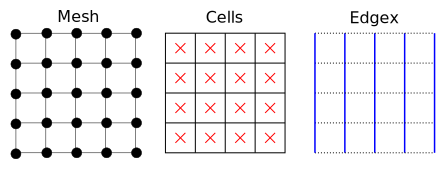
\includegraphics{./images/mesh.pdf}}
}
\hspace{10pt}
\subfloat[4-neighborhood stencil.\label{fig:ex1}]{
\resizebox{5cm}{!}{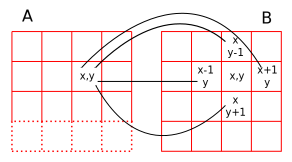
\includegraphics{./images/stencil1.pdf}}
}
\hspace{10pt}
\subfloat[2-neighborhood 2-entity stencil.\label{fig:ex2}]{
\resizebox{5cm}{!}{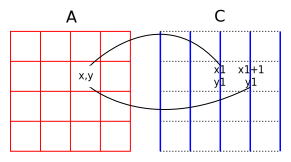
\includegraphics{./images/stencil2.pdf}}
}
\end{center}
\caption{(a) a Cartesian mesh and two kind of mesh entities, (b) an example of stencil kernel on cells, (c) an example of stencil kernel on two different entities of the mesh.}
\label{fig:gspmsp}
\end{figure}

% \begin{figure}[!h]\begin{center}
%   \resizebox{7cm}{!}{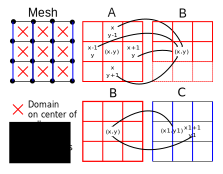
\includegraphics{./images/stencil.pdf}}
%   \caption{Examples of a stencil computations}
%   \label{fig:ex}
% \end{center}\end{figure}

A \emph{stencil kernel} computes the value of one data or a subpart of it (the kernel \emph{computation domain}) using a \emph{numerical expression} which takes as input one or more data.
For example, the stencil kernel illustrated in Figure~\ref{fig:ex1} computes $A$ using $B$, while the one in Figure~\ref{fig:ex2} computes $A$ using $C$. Thus, a stencil kernel is defined by its numerical expression, a set of input data (only one in the examples), and its unique output data, the result. 
The \emph{computation domain} is a subset of the mesh entities on which the output data is mapped. For example, in the first stencil, the computation of $A$ is performed on elements represented with full lines, while dotted elements are not computed. On the other hand, on the second computation, the computation domain of $A$ contains all the mesh entities on which it is mapped. This computation domain defines the elements over which the space loop iterates.

The numerical expression of a stencil kernel has the particularity to compute each element of the result independently using some elements of the inputs in a given neighborhood.
Accessed elements form a \emph{neighborhood} of the output known as the \emph{stencil shape}. For example, the stencil shape of the first computation in Figure~\ref{fig:ex1} contains direct neighbors on the right, left, top and bottom. Sometimes, the neighborhood can also access different mesh entities, as for example in Figure~\ref{fig:ex2}. Actually, in this computation, the neighborhood contains edges on the left and on the right of a cell. As an example, the numerical expression of the first example could be:
\begin{equation*} 
A(x,y) = B(x+1,y)+B(x-1,y)+B(x,y+1)+B(x,y-1),
\end{equation*}
and the numerical expression of the second kernel could be:
\begin{equation*} 
A(x,y) = A(x,y)+C(x1,y1)+C(x1+1,y1).
\end{equation*}

As it can be seen from these definitions, stencil kernels implementations share many properties from an algorithmic point of view that can be used to apply well known optimization and parallelization strategies.
Many solutions (languages or frameworks) thus propose to ease their programming by producing optimized and parallelized code from a simple description of the local computation to apply on each element.
These are further discussed in Sections~\ref{sect:related}.

%To resume, concepts used in this paper to define a stencil kernel are \emph{mesh}, \emph{mesh entities}, \emph{data}, \emph{computation domain}, \emph{numerical expression} and \emph{stencil shape}. 
While stencil kernels have been studied a lot, the formalization of real overall mesh-based numerical simulations is poorly studied and not exactly for the same kind of appication~\cite{Ragan-Kelley:2013:HLC:2491956.2462176}. Actually, paying attention to complex numerical simulations, it appears that most of them are composed of more than one stencil kernel, with one or more stencil shapes and of additional local computations. For example, we would like to formalize and parallelize a numerical simulation which chains the stencil kernels of Figures~\ref{fig:ex1} and~\ref{fig:ex2}. The next section formalizes concepts of \emph{stencil kernel}, \emph{local kernel} and \emph{multi-stencil program}.

%----------------------------------------
\subsection{A Multi-Stencil Formalization}
\label{sect:multistencil}
%----------------------------------------
This section introduces some formal definitions used in the rest of the paper.
Let $\Delta$ be the set of data of the simulation
A stencil kernel $s$ is defined as the quadruplet:
\begin{equation} 
s(R,w,exp,d),
\label{eq:st}
\end{equation}
where $R$ is a set of pairs $(r,n)$, with $r \in \Delta$ a data read by the computation, and $n$ the stencil shape (neighborhood) used to access $r$. The data written by the kernel is denoted $w \in \Delta$. $exp$ is the numerical expression of the stencil kernel. Finally the numerical expression is applied on the computation domain $d$.

For example, in Figure~\ref{fig:ex1}, assuming the computation domain (full lines) is $dc1$ and the stencil shape is $n1$, the stencil kernel can be defined as:
\begin{equation*}
R: \{(B,n1)\}, \quad w: A, \quad d: dc1,
\end{equation*}
\begin{equation*}
exp: A(x,y)=B(x+1,y)+B(x-1,y)+B(x,y+1)+B(x,y-1).
\end{equation*}
On the other hand, in the example of Figure~\ref{fig:ex2}, assuming the computation domain is $dc2$ and the stencil shape is $n2$, the stencil kernel is defined as:
\begin{equation*}
R: \{(C,n2),(A,local)\}, \quad w: A, \quad d: dc2,
\end{equation*}
\begin{equation*}
exp: A(x,y)=A(x,y)+C(x1,y1)+C(x1+1,y1).
\end{equation*}
One can notice that the input data $A$ is associated to the stencil shape $local$. This means that the stencil shape applied on $A$ is limited to the element with the exact same coordinate as the result element.

The specificities of kernels whose stencil shapes are all local makes it possible to apply specific optimizations.
We therefore provide a specific definition in this case.
A local (or auxiliary) kernel $l$ is defined as the quadruplet:
\begin{equation} 
l(R_l,w,exp,d),
\label{eq:loc}
\end{equation}
where $R_l$ is the set of input data locally accessed, and other parameters are the same as for normal stencil kernels.

We define a multi-stencil program as a sextuplet:
\begin{equation} 
\mathcal{MSP}(T,\mathcal{M},\mathcal{E},\mathcal{D},\Delta,\Gamma),
\label{eq:msp}
\end{equation}
where $T$ is the set of time iteration to run the simulation, $\mathcal{M}$ is the mesh of the simulation, $\mathcal{E}$ is the set of mesh entities, $\mathcal{D}$ is the set of computation domains used for computations, $\Delta$ is the set of data of the simulation, each one mapped onto a mesh entity, and finally $\Gamma$ is the set of computations. The set of computations $\Gamma$ is an ordered list of stencil and local kernels.
One can notice that this work, for now, is limited to a single mesh type for a given simulation.

% !!!!!!!!!!!! a mettre en plus court autre part !!!!!!!!!!!!!!!
%----------------------------------------
% \subsection{Parallelization techniques}
% \label{sect:parallel}
%----------------------------------------
% Three classical parallelization techniques are used in this paper and are described in this section, the data parallelism, the task parallelism, and the hybrid data and task parallelism. Those parallelization techniques are independent from the actual parallel hardware used.

% \paragraph{Data parallelism} The idea of this parallelization technique is to split, or partition, data on which computations are applied among available processors (or cores). Each processor then applies the same progam or instruction onto its subpart of data. Moreover, if a neighborhood information is needed from another processor communications or synchronizations are performed. 

% In the domain of numerical simulations, this technique is most of the time called a domain decomposition. This parallelization technique produce efficient programs up to thousands processors or cores, but on certain conditions. First, each subpart of data has to be big enough to overlap communication time. Second, the partitioning of data has to be balanced among processors. Thus, if this parallelization technique is clearly adequate to structured meshes, easy to balance, it is not for unstructured meshes or irregular structures where the amount of work is not heterogenous.

% \paragraph{Task parallelism} Another well known parallelization technique is to identify in a program the different tasks and which one are independant and can be launched concurrently. Most of the time, such a prallelization technique create a dependency directed acyclic graph (dependency dag) from a set of ordered tasks. Dependencies are found from read/write information for each task. Actually, if a task $i$ write a data $a$ and if a task $j$ read $a$, then $i$ has to be finished before $j$ is performed. From a dependency graph two different solutions are available. First, a static schedule of tasks is built, which could be a good solution if the tasks are regular, or use a dynamic scheduler to dynamically decide at runtime which task is executed on which processor.

% \paragraph{Hybrid parallelism} Finally, it is also possible to combine both those parallelization techniques to get what is called an hybrid parallelization. The interest of an hybrid parallelization is to bring another source of parallelism if limits of a given technique are reach.


%----------------------------------------
\section{MSL and MSCAC Overview }
\label{sect:mscac}
The solution proposed in this paper contains a domain specific language to describe a multi-stencil program, \ie an overall numerical simulation, and a compiler which successively parses the front-end language, transforms the internal representation, and finally dumps the representation to a component-based back-end code.

The proposed DSL, named MSL (\emph{Multi-Stencil Language}), is an agnostic descriptive language for multi-stencil simulations. Agnostic means that the description of a numerical simulation does not depend on implementation choices as, for example, the type of mesh (structured, unstructured), or its associated interfaces (how to define a stencil shape, etc.). Descriptive, on the other hand, means that the terminal states of the language grammar are (string) identifiers. As a result, MSL is not made to handle the expression of numerical computations, but only the description of a multi-stencil simulation, in a coarse-grain fashion. %Numerical computations are encapsulated in specific components that users have to develop. 
In a MSL description, six main sections are defined, as the six tuples of the definition of a multi-stencil program of Equation~\ref{eq:msp}.

\begin{figure}[t]
\begin{center}
\begin{tikzpicture}[remember picture,
  inner/.style={rectangle,rounded corners=3pt,thick,inner sep=5pt},
  outer/.style={rectangle,rounded corners=3pt,thick,inner sep=5pt}
  ]
  \node (MSL) {MSL};
  \node[outer,below=0.5 of MSL,draw=black] (MSCAC) {
    \begin{tikzpicture}
      \node [inner,draw=black,thick] (pars)  {Parser};
      \node [inner,draw=black,thick,below=0.5cm of pars] (MSC)  {MSC};
      \node [inner,below=0.5cm of MSC,draw=black,thick] (Dump)  {Dump};

      \draw[->] (pars) -- (MSC);
      \draw[->] (MSC) -- (Dump);
    \end{tikzpicture}
  };
  \node [below=0.5 of MSCAC] (CA) {Component-based runtime};
  \node [rotate=90,above left=0.5 of MSC] (CAid) {MSCAC};
  \draw[->] (MSL) -- (pars.north);
  \draw[->] (Dump.south) -- (CA);
\end{tikzpicture}
\caption{The three phases of the MSCAC compiler.}
\label{fig:mscac}
\end{center}
\end{figure}

As illustrated in Figure~\ref{fig:mscac}, the compiler, named MSCAC for \emph{Multi-Stencil Component Assembly Compiler}, is composed of three different phases. The first phase of the compiler is to \emph{parse} the MSL description. Second, the compiler analyzes and transforms the computation part of the description $\Gamma$, to an intermediate representation. This phase of compilation, called MSC, is responsible for the automatic parallelization of the overall numerical simulation. Finally, the parallel intermediate representation is dumped to an actual implementation of the parallel pattern of the simulation.

% As illustrated in Figure~\ref{fig:mscac}, the MS language compiler, called MSCAC for \emph{Multi-Stencil Component Assembly Compiler}, is composed of two different parts. First, the computation compiler, called \emph{MSC}, is responsible for the parallelization of computations and for its dump to a component assembly; second, the data compiler, called \emph{MSD}, handles a distributed data structure, data mapped onto it, and their relations with computations, as a final overall component assembly.

%In this paper are presented the language MSL, the MSC compilation phase, and the dump compilation phase. 
The parallelization techniques handled by MSC are \emph{data parallelism}, where data are splitted among processors or cores while applying a single program everywhere, and \emph{task parallelism} where the program is transformed into a dependency graph of tasks. From a dependency graph, different strategies can be used to schedule tasks, in other words to control their execution in a valid order. The MSC compiler presented in this paper handles the transformation of the dependency graph to a static scheduling.

The final phase of compilation, the dump, uses the static schedule of the tasks, created from $\Gamma$, and additionnal information on $T$, $\mathcal{M}$, $\Delta$, $\mathcal{E}$ and $\mathcal{D}$, given by the \emph{parser}, to produce a back-end solution which represents the parallel pattern or skeleton of the overall simulation. We could have propose a dump to OpenMP~\cite{660313}, however this paper presents a first contribution to dump a DSL to a component-based runtime. Component models, where a component represents a clear and independent functionnality of the application, have first been proposed in software engineering and have proved many times good properties for code re-use, separation of concerns, maintainability and productivity of codes. Those properties, on the other hand, are recurrent stated problems of parallel applications.

The back-end of the compiler builds a component assembly, that can be divided in two parts: the components implementing the actual computation and the static schedule, and the components needed to manage it, \ie the runtime support. A general view of this assembly is proposed in Figure~\ref{fig:mscac:assembly}; it is explained in details in Section~\ref{sect:component}. As illustrated in the figure, each component is linked to one or more tuple of the multi-stencil program definition: \emph{DDS} component represents $\mathcal{M}$ and $\mathcal{E}$; \emph{Data} component represents $\Delta$ and $\mathcal{D}$; \emph{Time} component represents $T$, and \emph{Computations} component (which is generated by MSC) represents $\Gamma$.

The final back-end component assembly is a ready-to-fill parallel structure where the user has to write computation codes described in the MSL description. To write those computations, interfaces of the choosen implementation have to be used. For example, the back-end evaluated in this paper uses the distributed data structure proposed in SkelGIS library~\cite{CPE:CPE3494}. A work in progress replaces this DDS component by another one making use of Global Arrays~\cite{Nieplocha:2006:AAP:1125980.1125985}.

\begin{figure}[t]
\begin{center}
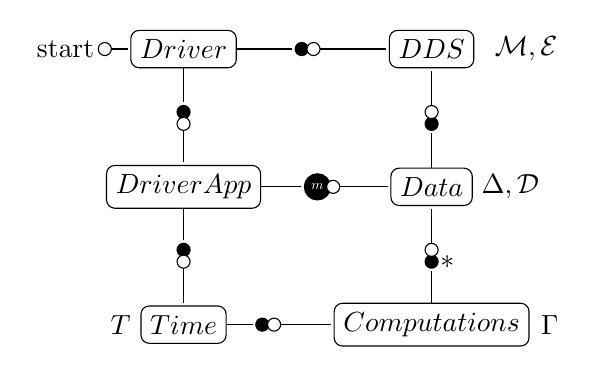
\begin{tikzpicture}[shorten >=1pt, node distance=2cm, on grid, auto]
   \node[component] (D) at (0,0) {$Driver$};
   \node[provide] (Dp) at (-1,0) {};
   \node (Ds) at (-1.5,0) {start};
   \node[use,right=1.5cm of D] (Du1) {};
   \node[use,below=0.8cm of D] (Du2) {};

   \node[provide,below=0.15 of Du2] (DAp) {};
   \node[component,below=0.8cm of DAp] (DA) {$DriverApp$};
   \node[use,right=1.7cm of DA] (DAu1) {$m$};
   \node[use,below=0.8cm of DA] (DAu2) {};

   \node[provide,below=0.15 of DAu2] (Tp) {};
   \node[component,below=0.8cm of Tp] (T) {$Time$};
   \node[use,right=1cm of T] (Tu) {};
   \node[left=0.8cm of T] (tt) {$T$};

   \node[provide,right=0.15 of Tu] (Cp) {};
   \node[component,right=2cm of Cp] (C) {$Computations$};
   \node[use,above=0.8cm of C] (Cu) {};
   \node[right=0.2cm of Cu] (star) {$*$};
   \node[right=1.5cm of C] (gamma) {$\Gamma$};

   \node[provide,right=0.2 of DAu1] (Datap1) {};
   \node[provide,above=0.15 of Cu] (Datap2) {};
   \node[component,above=0.8cm of Datap2] (Data) {$Data$};
   \node[use,above=0.8cm of Data] (Datau) {};
   \node[right=1cm of Data] (delta) {$\Delta,\mathcal{D}$};

   \node[provide,right=0.15 of Du1] (DDSp1) {};
   \node[provide,above=0.15 of Datau] (DDSp2) {};
   \node[component,above=0.8cm of DDSp2] (DDS) {$DDS$};
   \node[right=1.2cm of DDS] (m) {$\mathcal{M},\mathcal{E}$};
 
  \path[-]
    (Dp) edge node {} (D)
    (D) edge node {} (Du1)
        edge node {} (Du2)
    (DDSp1) edge node {} (DDS)
    (DA) edge node {} (DAu1)
           edge node {} (DAu2)
    (DAp) edge node {} (DA)
    (Tp) edge node {} (T)
    (T)  edge node {} (Tu)
    (Cp) edge node {} (C)
    (C) edge node {} (Cu)
    (Datap2) edge node {} (Data)
    (Datap1) edge node {} (Data)
    (Data) edge node {} (Datau)
    (DDSp2) edge node {} (DDS);
\end{tikzpicture}
\caption{MSCAC Component Assembly Back-End Overview.}
\label{fig:mscac:assembly}
\end{center}
\end{figure}

% This paper presents the MS language and the MSC part of the compiler. The MSC compiler produces a static scheduling of the set of computations, ready to dump to a parallel language, such as OpenMP~\cite{660313} or HPF~\cite{219857}, but also ready to dump to a component assembly which is the main contribution of this work.

% \begin{figure*}
% \begin{center}
% \begin{tikzpicture}[shorten >=1pt, node distance=2cm, on grid, auto]
%    \node[component] (D) at (0,0) {$Driver$};
%    \node[provide] (Dp) at (-1,0) {};
%    \node (Ds) at (-1.5,0) {start};
%    \node[use] (Du1) at (1,0.5) {};
%    \node[use] (Du2) at (1,-0.5) {};

%    \node[component,right=1cm of Du2] (DA) {$DriverApp$};
%    \node[use] (DAu1) at (3.5,0) {$m$};
%    \node[use] (DAu2) at (3.5,-1) {};

%    \node[component] (T) at (4.5,-1) {$Time$};
%    \node[use,right=1cm of T] (Tu) {};
%    \node[component,right=2cm of Tu] (C) {$Computations$};
%    \node[use,right=2cm of C] (Cu) {};
%    \node[below=0.2cm of Cu] (star) {$*$};

%    \node[component,right=8cm of DAu1] (Data) {$Data$};
%    \node[use,right=1cm of Data] (Datau) {};

%    \node[component,right=13cm of Du1] (DDS) {$DDS$};
 
%   \path[-]
%     (Dp) edge node {} (D)
%     (D.east) edge node {} (Du1)
%       edge node {} (Du2)
%     (Du1) edge node {} (DDS.west)
%     (Du2) edge node {} (DA)
%     (DA.east) edge node {} (DAu1)
%       edge node {} (DAu2)
%     (DAu1) edge node {} (Data.west)
%     (DAu2) edge node {} (T)
%     (T) edge node {} (Tu)
%     (Tu) edge node {} (C)
%     (C) edge node {} (Cu)
%     (Cu) edge node {} (Data.west)
%     (Data) edge node {} (Datau)
%     (Datau) edge node {} (DDS.west);
% \end{tikzpicture}
% \caption{Shape of the generated component assembly.}
% \label{fig:assembly}
% \end{center}
% \end{figure*}

% It has to be noticed that in this paper, the MSD compiler is a first adhoc version which works for a precise distributed data structure, the SkelGIS library~\cite{HeleneLS13,HeleneLS14,HeleneEuroPar14,CPE:CPE3494}. However, using the system of python string templates~\footnote{\url{https://docs.python.org/2/library/string.html}} to define the component assembly part which manages data, it is already possible to use another distributed data structure, as for example Global Arrays~\cite{Nieplocha:2006:AAP:1125980.1125985}. This part of the compiler takes place in a larger research project to propose domain decomposition skeletons using component models.

% The overall compiler MSCAC produces a ready-to-fill component-based parallel structure of the simulation. In this final component assembly, it is needed to write computation components, using interfaces of the distributed data structure choosen by MSD. Thus, this work is complementary to stencil compilers or to distributed data structure solutions.

%----------------------------------------
\section{Language and Parallelization Description}
\label{sect:msmsc}
%----------------------------------------
\subsection{MS language}
%----------------------------------------
The MS language (MSL) is an agnostic descriptive language for multi-stencil simulations. Agnostic means that no knowledge on the mesh type and the neighborhood description of stencil computations are needed in the language. As the language consists in a description of the simulation, without any computation details and programming details, and as no computation is directly done from the language, this language is also called a descriptive language. It is composed of five description sections:
\begin{enumerate}
\item meshes description;
\item domains description;
\item data description;
\item time loop description;
\item computations description.
\end{enumerate}

This paper deals with the MSC compiler which only needs the three last enumerations above. For this reason we describe in the rest of this section MSL for data, time loop and computations descriptions.

\paragraph{Data description} Data description starts with the tag $data:$. Each line after this tag represents a single data description. This description is composed of an identification name, and the domain identification name it is applied on.

\begin{lstlisting}[basicstyle=\footnotesize,mathescape,frame=single,language=C++]
data:
  name_id,domain_id
\end{lstlisting}

\paragraph{Time description} The time of a numerical simulation consists in a set of iterations. The end of the simulation time can be controlled by a convergence function or by a manual configuration of the number of iteration. In this first version of MSL, the iteration number is handled.

\begin{lstlisting}[basicstyle=\footnotesize,mathescape,frame=single,language=C++]
time:nb_iteration
\end{lstlisting}

\paragraph{Computations description} The most important part of MSL is the description of the computations of the simulation. The language follows the definitions given in Section~\ref{sect:multistencil}. Thus, the description of a computation consists of a type of computation, an identification name of the computation, a set of identifiers for the data read by the computation, a single identifier for the data written by the computation. Moreover, if the type of computation is a stencil, a neighborhood identifier is needed.

\begin{lstlisting}[basicstyle=\footnotesize,mathescape,frame=single,language=C++]
computations:
  type:name_id({read1_id,read2_id,...},
 	    written_id[,neighborhood_id])
\end{lstlisting}

%----------------------------------------
\subsection{MSC compiler}
%----------------------------------------
The MSC compiler, which is a subpart of the overall compiler MSCAC, performs an algorithm composed of six main steps described bellow:

\begin{enumerate}
\item creation of $\Gamma$, the ordered list of computations, from the MSL input file;
\item creation of $\Gamma_{data}$ to insert synchronizations in the ordered list of computations;
\item creation of the dependency graph $\Gamma_{hybrid}$;
\item transform $\Gamma_{hybrid}$ to a minimal series-parallel graph $\Gamma_{msp}$;
\item creation of the series-parallel tree decomposition $\Gamma_{tsp}$;
\item dump $\Gamma_{tsp}$ to a component assembly.
\end{enumerate}

\paragraph{Creation of the ordered list of computations} This step of the MSC compiler parse the MSL input file which describes the simulation. From the ordered lines of computations, it builds the ordered list of computations $\Gamma$ to perform in the simulation.

\paragraph{Creation of the synchronized ordered list of computations} From the ordered list of computations $\Gamma$ it is possible to detect needed synchronizations if a \emph{data parallelization} \textbf{(PB: to explain !!!)} is performed on the simulation. A synchronization is needed each time a data read by a stencil computation has been written by a previous computation different from a boundary computation. Actually, as a stencil computation needs neighborhood values, in a domain decomposition values computed by different processors or cores are needed.

\paragraph{Creation of the dependency graph} From the synchronized ordered list of computations $\Gamma_{data}$, a dependency graph can be build. A dependency exists between two computations (including synchronizations) if and only if a data read has been written by a previous computation in $\Gamma_{data}$. Nodes of the dependency graph are computations and synchronizations, while edges are dependencies between them. $\Gamma_{hybrid}$ is a directed acyclic graph (\emph{dag}) as it is build from an ordered list.

\paragraph{Transformation to a minimal series-parallel graph} As it has been shown in~\cite{Valdes:1979:RSP:800135.804393}, the transitive reduction of a dag is a minimal series-parallel graph if and only if the forbidden \emph{N-shape} is not found in the graph. To transform $\Gamma_{hybrid}$ to the minimal series-parallel graph $\Gamma_{msp}$, a BFS algorithm is applied to build a complete bipartite between two levels of $\Gamma_{hybrid}$~\cite{Mitchell:2004:CMV:1082101.1082117}.

\paragraph{Creation of a tree decomposition} As shown in different works~\cite{Valdes:1979:RSP:800135.804393,Schoenmakers95anew}, from a minimal series-parallel graph a tree decomposition can be built. A series-parallel tree decomposition consists in the decomposition of the graph as a set of \emph{sequences} and \emph{parallel} sections in a tree. 

\paragraph{Dump to a component assembly} From the series-parallel tree decomposition $\Gamma_{tsp}$ can be built a program using any parallel language containing \emph{parallel sections} and \emph{sequences of instructions} such as OpenMP~\cite{660313}, HPF~\cite{219857}, UPC~\cite{El-Ghazawi:2006:UUP:1188455.1188483} etc. In this paper we study the dump of $\Gamma_{tsp}$ to a component assembly which needs the introduction of \emph{control components} described in the next section.

For more details on MSC, a full description of the compilation is described in~\cite{}.

%----------------------------------------
\subsection{Example}
%----------------------------------------
In this Section we give an example of an input file written with MSL, the $\Gamma_{tsp}$ series-parallel tree decomposition computed and the final component dump.

The input MSL file, shown in Figure~\ref{fig:msinput} is composed of nine computations and ten data.

\begin{figure}[h!]
\begin{lstlisting}[basicstyle=\footnotesize,mathescape,frame=single,language=C++]
data:
  a,d1
  b,d1
  c,d2
  d,d2
  e,d3
  f,d1
  g,d3
  h,d2
  i,d1
  j,d2
time:500
computations:
  local:c0({a},b)
  stencil:c1({b},c,n1)
  local:c2({c},d)
  local:c3({c},e)
  stencil:c4({d},f)
  local:c5({e},g)
  local:c6({f},h)
  local:c7({g,h},i)
  stencil:c8({i},j,n1)
\end{lstlisting}
\caption{Example of MSL input file}
\label{fig:msinput}
\end{figure}

The first step of the compilation is to build the synchronized ordered list of computations $\Gamma_{data}$. In this example each stencil computation actually needs a synchronization. For example, the stencil computation $c_1$ read the data $b$ which has been written by the computation $c_0$. For this reason the sublist $[c_0,c_1]$ of $\Gamma$ is transformed to the sublist $[c_0,sync_1,c_1]$ in $\Gamma_{data}$. The new computation $sync_1$ read and write $b$. As a result a dependency is kept between $sync_1$, and $c_1$. The same is performed for the stencils $c_4$ and $c_8$.

Once the synchronized list $\Gamma_{data}$ is obtained, the dependency graph $\Gamma_{hybrid}$ is built and illustrated in Figure~\ref{fig:hyb}. Each computation (and synchronization) is a node of the graph, while each edge represent a read/write data dependency between computations.

\begin{figure}[h!]
\begin{center}
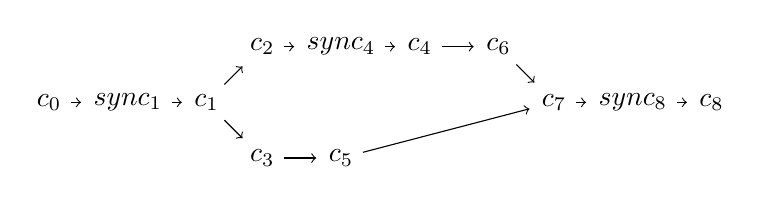
\begin{tikzpicture}[shorten >=1pt, node distance=2cm, on grid, auto]
   \node (c0) at (0,0) {$c_0$};
   \node[right=1 of c0] (sy1) {$sync_1$};
   \node[right=1 of sy1] (c1) {$c_1$};
   \node[above right=1 of c1] (c2) {$c_2$};
   \node[below right=1 of c1] (c3) {$c_3$};
   \node[right=1 of c2] (sy4) {$sync_4$};
   \node[right=1 of c3] (c5) {$c_5$};
   \node[right=1 of sy4] (c4) {$c_4$};
   \node[right=1 of c4] (c6) {$c_6$};
   \node[below right=1 of c6] (c7) {$c_7$};
   \node[right=1 of c7] (sy8) {$sync_8$};
   \node[right=1 of sy8] (c8) {$c_8$};
 
  \path[->]
    (c0) edge node {} (sy1)
    (sy1) edge node {} (c1)
    (c1)  edge node {} (c2)
          edge node {} (c3)
    (c2) edge node {} (sy4)
    (sy4) edge node {} (c4)
    (c4) edge node {} (c6)
    (c3) edge node {} (c5)
    (c5) edge node {} (c7)
    (c6) edge node {} (c7)
    (c7) edge node {} (sy8)
    (sy8) edge node {} (c8);
\end{tikzpicture}
\caption{$\Gamma_{hybrid}$ of Figure~\ref{fig:msinput}}
\label{fig:hyb}
\end{center}
\end{figure}

After a set of transformation briefly explained in the previous Section, a series-parallel tree decomposition $\Gamma_{tsp}$ is obtained and illustrated in Figure~\ref{fig:canon}.

\begin{figure}[h!]
\begin{center}
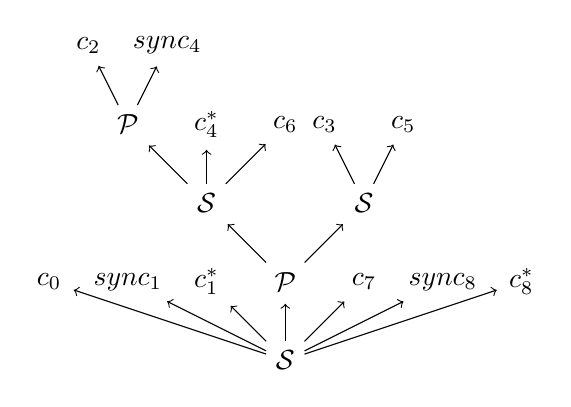
\begin{tikzpicture}[shorten >=1pt, node distance=2cm, on grid, auto]
   \node[] (s0) at (0,0) {$\mathcal{S}$};
   \node[] (c0) at (-3,1) {$c_0$};
   \node[] (star1) at (-2,1) {$sync_1$};
   \node[] (c1) at (-1,1) {$c_1^*$};

   \node[] (p0) at (0,1) {$\mathcal{P}$};
   \node[] (s1) at (-1,2) {$\mathcal{S}$};
   \node[] (p1) at (-2,3) {$\mathcal{P}$};
   \node[] (c4) at (-1,3) {$c_4^*$};
   \node[] (c6) at (-0,3) {$c_6$};
   \node[] (c2) at (-2.5,4) {$c_2$};
   \node[] (star4) at (-1.5,4) {$sync_4$};
   \node[] (s2) at (1,2) {$\mathcal{S}$};
   \node[] (c3) at (0.5,3) {$c_3$};
   \node[] (c5) at (1.5,3) {$c_5$};

   \node[] (c7) at (1,1) {$c_7$};
   \node[] (star8) at (2,1) {$sync_8$};
   \node[] (c8) at (3,1) {$c_8^*$};
 
  \path[->]
    (s0) edge node {} (c0)
         edge node {} (star1)
         edge node {} (c1)
         edge node {} (p0)
         edge node {} (c7)
         edge node {} (star8)
         edge node {} (c8)
    (p0) edge node {} (s1)
         edge node {} (s2)
    (s1) edge node {} (p1)
         edge node {} (c4)
         edge node {} (c6)
    (p1) edge node {} (c2)
         edge node {} (star4)
    (s2) edge node {} (c3)
         edge node {} (c5);
  \end{tikzpicture}
\caption{$\Gamma_{tsp}$ of Figure~\ref{fig:hyb}.}
\label{fig:canon}
\end{center}
\end{figure}



%----------------------------------------
\section{A Component based Back-End}
\label{sect:component}
%-------------------------------------
\subsection{Component models}
A \textit{component} is an independent object which represents a functionnality of an application, and which is associated to a set of \textit{interfaces} used to plug an instance of a component with other ones. The object composed of multiple component instances linked together through their interfaces is called a component assembly. As a result, a component assembly is the code of an entire application represented as a set of splitted functionnalities. Such software engineering model is known to increase \textit{code re-use} and \textit{productivity}, as one component can be used in different applications, but also \textit{maintainability} and \textit{scalability}, as functionnalities of an application are clearly splitted in different and independent components. More recently, component models have been studied to write HPC applications such as $L^2C$~\cite{} (Low Level Component Model) and CCA~\cite{} (Common Component Architecture).

In the rest of this paper, the component model $L^2C$ is considered and used by the solution. A component is defined as
\begin{equation}
C(I,F),
\end{equation}
where $I$ is a set of available interfaces for the given component, and $F$ is the set of functions to answer the functionnality of the component. A component instance, as for an object, is the actual creation of the component, and more than one instance can be created. The components of $L^2C$ are limited to a few interfaces without the introduction of overheads. In this paper we are interested in four types of interfaces. The three first one are \textit{use} and \textit{provide} interfaces (Figure~\ref{AB}) to use a functionnality provided by another component instance, and \textit{use-multiple} interface (Figure~\ref{ABC}) to use a vector of functionnalities provided by a set of component instances. A condensed notation of a use-multiple is given in the Figure~\ref{ABCbis}. 

\begin{figure}[h!]
\begin{center}
  \subfigure[][$A$ uses $B$ and $A$ uses $C$]{
  \begin{tikzpicture}[shorten >=1pt, node distance=2cm, on grid, auto]
   \node[component] (A) at (0,0) {$A$};
   \node[component] (B) at (2,+0.5) {$B$};
   \node[component] (C) at (2,-0.5) {$C$};
 
  \path[-]
    ([yshift=1ex]A.east) edge [connection] (B.west)
    ([yshift=-1ex]A.east) edge [connection] (C.west);
  \end{tikzpicture}
  \label{AB}
  }
  \hspace{2cm}
  \subfigure[][$A$ uses multiple $B$ instances]{
  \begin{tikzpicture}[shorten >=1pt, node distance=2cm, on grid, auto]
   \node[component] (A) at (0,0) {$A$};
   \node[component] (B) at (2,+0.5) {$B_1$};
   \node[component] (C) at (2,-0.5) {$B_2$};
 
  \path[-]
    (A.east) edge [connection] node {} (B.west)
             edge [connection] node {} (C.west);

  \end{tikzpicture}
  \label{ABC}
  }
  \hspace{2cm}
  \subfigure[][$A$ uses multiple $B$ instances (condensed notation)]{
  \begin{tikzpicture}[shorten >=1pt, node distance=2cm, on grid, auto]
   \node[component] (A) at (0,0) {$A$};
   \node[component] (B) at (2,0) {$B$};
 
  \path[-]
    (A.east) edge [connection] node {1,n} (B.west);

  \end{tikzpicture}
  \label{ABCbis}
  }
  \caption{$L^2C$ use-provide and use-multiple interfaces}
  \label{interfaces}
\end{center}
\end{figure}

An instance $i$ of a component has the same properties than the component it is instanciated from, but it is also asociated to a resource $r$ (a core, a thread etc.) of the set of all available resources $R$.
\begin{equation}
C_i(I,F,r)
\end{equation}
A component assembly represents the application as a set of component instances and the composition of those instances through their interfaces. A component assembly is defined as
\begin{equation}
\alpha (\mathcal{C},L,R),
\end{equation}
where $\mathcal{C}$ is the set of component instances used, $L$ is the set of links between interfaces of component instances, and $R$ is the set of available resources. The component assembly of $L^2C$ offers a way to write an assembly for each MPI process, and to connect some of their components by MPI communicators. This connection is an \textit{MPI interface}. In the rest of this paper we consider a broader interface called \textit{synchronization}, which corresponds to the MPI interface of $L^2C$ but which could also be a \textit{thread synchronization} instead.

Using those four interfaces (use, use-multiple, provide and synchronization), it is possible to write an application with medium-grain components, enough fine to keep efficiency and to stay close to the execution model, and enough coarse to take advantage of components. The efficiency of $L^2C$ has been proved, while increasing the productivity and maintainability of HPC applications, but moreover it has also been shown that the protability of such component-based HPC application is improved~\cite{}.

%-------------------------------------
\subsection{Stencil program parallelization using components}
In this section is studied the parallelization of a numerical simulation using the given definitions of a component, an assembly and four interfaces. First, the different parallelization techniques explained in the Section~\ref{sect:parall} are translated to component-based parallel assemblies, and an approximation of the general case is discussed for the solution presented in this paper. In the rest of this section, the following example of dependencies is used 
\begin{equation}
A<((B<D) \parallel C)<E \ll A'<((B'<D') \parallel C'),
\label{eq:dep}
\end{equation}
 where $A,B,C,D,E,A',B',C',D'$ are numerical computations. %In this example, $\parallel$ is a binary expression which means that a parallel execution of the right and left computations is possible. It is equivalent to $\not>$. 
This example, can be represented as a directed acyclic graph as in the Figure~\ref{example}.

\begin{figure}[h!]
\begin{center}
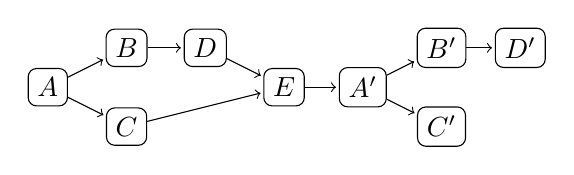
\begin{tikzpicture}[shorten >=1pt, node distance=2cm, on grid, auto]
   \node[component] (A) at (0,0) {$A$};
   \node[component] (B) at (1,+0.5) {$B$};
   \node[component] (C) at (1,-0.5) {$C$};
   \node[component] (D) at (2,+0.5) {$D$};
   \node[component] (E) at (3,0) {$E$};
   \node[component] (AA) at (4,0) {$A'$};
   \node[component] (BB) at (5,+0.5) {$B'$};
   \node[component] (CC) at (5,-0.5) {$C'$};
   \node[component] (DD) at (6,+0.5) {$D'$};
 
  \path[->]
    (A) edge node {} (B)
        edge node {} (C)
    (B) edge node {} (D)
    (D) edge node {} (E)
    (C) edge node {} (E)
    (E) edge node {} (AA)
    (AA) edge node {} (BB)
        edge node {} (CC)
    (BB) edge node {} (DD);
  \end{tikzpicture}
  \caption{Dependencies example~(\ref{eq:dep}) represented as a DAG.}
  \label{example}
\end{center}
\end{figure}

%---------
%---------
\paragraph{Coarse- and fine-grain data parallelism.} 
As explained in the Section~\ref{sect:parall}, to apply coarse-grain data parallelism on numerical simulations, a domain decomposition (or graph partitioning) has to be done on the mesh and also on the data mapped on it. When this important step is solved, the same program can be applied on each subpart of the data, on the different resources. In addition to this, a set of synchronizations are needed between the resources at each time step to compute the neighborhood $\mathcal{N}$ correctly. When using a component model, the computing part of the application, which is called for each time step, can be seen as a component assembly which is duplicated on different resources, which is possible using $L^2C$ for example. However, it is needed to classify computations in the component assembly to identify when synchronizations are needed (denoted $\ll$ in the Section~\ref{sect:dep}). For this reason, a \textit{sequence} component $SEQ$, which uses one after the other a set of computation components, is defined as 
\begin{equation}
SEQ(\{provide,use-multiple\},\{sequence\}).
\end{equation} 
Thus, the \textit{sequence} function (represented in the Algorithm~(\ref{alg:seq})) is responsible for the loop which calls as much \textit{uses} as the number of components connected to the \textit{use-multiple}. In addition to this, a \textit{synchronized sequence} component $SSEQ$, which uses one after the other a set of computation components, but which also proceeds synchronizations between them, is defined as 
\begin{equation}
SSEQ(\{provide,use-multiple, synchronization\},\{ssequence\}).
\end{equation}
In this case, the \textit{ssequence} function (represented in the Algorithm~(\ref{alg:sseq})) is responsible for a loop of two steps, first a synchronization step, second a use step. Finally, each numerical computation is represented by a component 
\begin{equation}
K(\{provide\},\{compute\}),
\end{equation}
 where the function \textit{compute} (represented in the Algorithm~(\ref{alg:comp})) is responsible for the sapce loop and the numerical computation on each element of the mesh.

\begin{center}
\begin{minipage}[t]{7cm}
  \vspace{0pt} 
 \begin{algorithm}[H]
 \ForAll{component $cp$ to use}{
 use the provide interface of $cp$
 }
 \caption{sequence function}
 \label{alg:seq}
 \end{algorithm}
 \end{minipage}%
 \hspace{0.5cm}
\begin{minipage}[t]{7cm}
  \vspace{0pt}
 \begin{algorithm}[H]
 \ForAll{component $cp$ to use}{
 synchronizations\\
 use the provide interface of $cp$
 }
 \label{alg:sseq}
 \caption{ssequence function}
 \end{algorithm}
 \end{minipage}%
\end{center}

%\begin{minipage}[t]{5cm}
 % \vspace{0pt}
 \begin{center}
 \begin{algorithm}[H]
 \ForAll{elements $d$ in $D$}{
 $w(d)=e(R(d),R(\mathcal{N}(d)))$
 }
 \caption{compute function}
 \label{alg:comp}
 \end{algorithm}
 \end{center}
%\end{minipage}%
Using the three components $SSEQ$, $SEQ$, and $K$, the component assembly of the dependencies~(\ref{eq:dep}) is represented in the Figure~~\ref{exdataparall}. One can notice, in this Figure, that the parallel dependencies ($\parallel$) are lost. However, in a SPMD parallelization, the parallelism is obtained from executing the same program on different part of the data. As a result, a correct sequence of computations is sufficient to expose coarse-grain data parallelism.
%---------
\begin{figure}[h!]
\begin{center}
\begin{tikzpicture}[shorten >=1pt, node distance=2cm, on grid, auto]
  \node[component] (SSEQ) at (0,0) {$SSEQ$};
  \node (sync) at (4,0) {Synchronizations};
  \node[component] (SEQ1) at (-2.5,-1) {$SEQ$};
  \node[component] (SEQ2) at (2.5,-1) {$SEQ$};
  \node[component] (A) at (-4,-2) {$A$};
  \node[component] (B) at (-3,-2) {$B$};
  \node[component] (C) at (-2,-2) {$C$};
  \node[component] (D) at (-1,-2) {$D$};
  \node[component] (E) at (0,-2) {$E$};
  \node[component] (AA) at (1,-2) {$A'$};
  \node[component] (BB) at (2,-2) {$B'$};
  \node[component] (CC) at (3,-2) {$C'$};
  \node[component] (DD) at (4,-2) {$D'$};
 
  \path[-]
    (SSEQ) edge [connection] node {} (SEQ1)
           edge [connection] node {} (SEQ2)
           edge [mpiconn] node {} (sync)
    (SEQ1) edge [connection] node {} (A)
           edge [connection] node {} (B)
           edge [connection] node {} (C)
           edge [connection] node {} (D)
           edge [connection] node {} (E)
    (SEQ2) edge [connection] node {} (AA)
           edge [connection] node {} (BB)
           edge [connection] node {} (CC)
           edge [connection] node {} (DD);

  \end{tikzpicture}
\caption{Example assembly for coarse- and fine-grain data parallelism}
\label{exdataparall}
\end{center}
\end{figure}
The overall computation assembly of an SPMD numerical simulation is composed of a duplication of the computation (or dependencies) assembly described above. Each duplication is applied on an available resource as illustrated in the Figure~\ref{overall}. In the rest of this paper, this overall computation assembly of an SPMD application (coarse-grain data parallelism) is represented as a single computation assembly, and the $SSEQ$ component indicate where the synchronizations are needed.

%---------
\begin{figure}[h!]
\begin{center}
\begin{tikzpicture}[shorten >=1pt, node distance=2cm, on grid, auto]
  \node[smallcp] (SSEQ) at (0,0) {$SSEQ$};
  \node (sync) at (3.5,0) {Synchronizations};
  \node[smallcp] (SEQ1) at (-1.5,-1) {$SEQ$};
  \node[smallcp] (SEQ2) at (1.5,-1) {$SEQ$};
  \node[smallcp] (A) at (-2.5,-2) {$A$};
  \node[smallcp] (B) at (-2,-2) {$B$};
  \node[smallcp] (C) at (-1.5,-2) {$C$};
  \node[smallcp] (D) at (-1,-2) {$D$};
  \node[smallcp] (E) at (-0.5,-2) {$E$};
  \node[smallcp] (AA) at (0.5,-2) {$A'$};
  \node[smallcp] (BB) at (1.1,-2) {$B'$};
  \node[smallcp] (CC) at (1.9,-2) {$C'$};
  \node[smallcp] (DD) at (2.5,-2) {$D'$};
  \draw [resource] (-3,-2.5) rectangle +(6cm, 3cm);
  \node (R1) at (0,-3) {r1};

  \node[smallcp] (SSEQ2) at (7,0) {$SSEQ$};
  \node[smallcp] (SEQ3) at (5.5,-1) {$SEQ$};
  \node[smallcp] (SEQ4) at (8.5,-1) {$SEQ$};
  \node[smallcp] (A2) at (4.5,-2) {$A$};
  \node[smallcp] (B2) at (5,-2) {$B$};
  \node[smallcp] (C2) at (5.5,-2) {$C$};
  \node[smallcp] (D2) at (6,-2) {$D$};
  \node[smallcp] (E2) at (6.5,-2) {$E$};
  \node[smallcp] (AA2) at (7.5,-2) {$A'$};
  \node[smallcp] (BB2) at (8.1,-2) {$B'$};
  \node[smallcp] (CC2) at (8.9,-2) {$C'$};
  \node[smallcp] (DD2) at (9.5,-2) {$D'$};
  \draw [resource] (4,-2.5) rectangle +(6cm, 3cm);
  \node (R2) at (7,-3) {r2};
 
  \path[-]
    (SSEQ) edge [connection] node {} (SEQ1)
           edge [connection] node {} (SEQ2)
           edge [mpiconn] node {} (sync)
    (SEQ1) edge [connection] node {} (A)
           edge [connection] node {} (B)
           edge [connection] node {} (C)
           edge [connection] node {} (D)
           edge [connection] node {} (E)
    (SEQ2) edge [connection] node {} (AA)
           edge [connection] node {} (BB)
           edge [connection] node {} (CC)
           edge [connection] node {} (DD)
    (SSEQ2) edge [connection] node {} (SEQ3)
           edge [connection] node {} (SEQ4)
           edge [mpiconn] node {} (sync)
    (SEQ3) edge [connection] node {} (A2)
           edge [connection] node {} (B2)
           edge [connection] node {} (C2)
           edge [connection] node {} (D2)
           edge [connection] node {} (E2)
    (SEQ4) edge [connection] node {} (AA2)
           edge [connection] node {} (BB2)
           edge [connection] node {} (CC2)
           edge [connection] node {} (DD2);

  \end{tikzpicture}
\caption{Overall SPMD computation assembly of the example~(\ref{eq:dep}) on two resources.}
\label{overall}
\end{center}
\end{figure}

But the assembly obtained from the instanciation of $SEQ$, $SSEQ$, and $K$ does not only expose coarse-grain data parallelism. Actually, the generic notation of a computation component $K$, which represents a numerical computation, is important to identifiy the different computations of a numerical simulation as different functionnalities of the program, but in addition to this, exposing a computation as a component, also exposes the fine-grain data parallelism level. In fact, a numerical computation is nothing more than a loop (or a nested loop) on the mesh elements and a numerical expression to compute (Algorithm~(\ref{alg:comp})). As a result a computation component is ideal to introduce SIMD and SIMT parallelism.

The general case of assembly to introduce coarse- and fine-grain data parallelism in numerical simulations is represented in the Figure~\ref{dataparall}.

\begin{figure}[h!]
\begin{center}
\begin{tikzpicture}[shorten >=1pt, node distance=2cm, on grid, auto]
   \node[component] (SSEQ) at (0,0) {SSEQ};
   \node[component] (SEQ) [right=of SSEQ] {SEQ};
   \node[component] (K) [right=of SEQ] {K};
 
  \path[-]
    (SSEQ)  edge [connection] node {1,n} (SEQ)
            edge [mpiconn] node {} (-1,0)
    (SEQ)	 edge [connection] node {1,n}	(K);
\end{tikzpicture}
\caption{General assembly description for coarse- and fine-grain data parallelism}
\label{dataparall}
\end{center}
\end{figure}
%---------

%---------
%---------
\paragraph{Data and task parallelism}
As also explained in the Section~\ref{sect:parall}, to apply task parallelism to numerical simulations, it is needed to identify the different tasks of the application and their dependencies. With the introduction of $SSEQ$, $SEQ$, and $K$ components, a part of this work is already done. Actually, each computation component $K$ represents a task. However, to be able to express all dependencies between computations, the $PAR$ component is defined as 
\begin{equation}
PAR(\{provide,use-multiple\},\{parallel\}),
\end{equation}
 and corresponds to the expression $\parallel$ or $\not<$. The function $parallel$ creates a thread for each component to use and join all threads at the end.

\begin{algorithm}[H]
 \ForAll{component $cp$ to use}{
 create thread $t$
 $t$ uses the provide interface of $cp$
 }
 join all threads
 \label{alg:par}
 \caption{parallel function}
 \end{algorithm}

\medskip
In addition to this, a composition of the components $SSEQ$, $SEQ$, $PAR$ and $K$ is needed to be able to represent complex dependencies. For example, the example dependencies~(\ref{eq:dep}) is represented in the Figure~\ref{exallparall}.
%---------
\begin{figure}[h!]
\begin{center}
\begin{tikzpicture}[shorten >=1pt, node distance=2cm, on grid, auto]
  \node[component] (SSEQ) at (0,0) {$SSEQ$};
  \node[component] (SEQ1) at (-2.5,-1) {$SEQ$};
  \node[component] (SEQ2) at (2.5,-1) {$SEQ$};
  \node[component] (A) at (-3.5,-2) {$A$};
  \node[component] (E) at (-1.5,-2) {$E$};
  \node[component] (PAR1) at (-2.5,-2) {$PAR$};
  \node[component] (AA) at (2,-2) {$A'$};
  \node[component] (PAR2) at (3,-2) {$PAR$};
  \node[component] (SEQ3) at (-3,-3) {$SEQ$};
  \node[component] (C) at (-2,-3) {$C$};
  \node[component] (SEQ4) at (2.5,-3) {$SEQ$};
  \node[component] (CC) at (3.5,-3) {$C$};
  \node[component] (B) at (-3.5,-4) {$B$};
  \node[component] (D) at (-2.5,-4) {$D$};
  \node[component] (BB) at (2,-4) {$B$};
  \node[component] (DD) at (3,-4) {$D$};
 
  \path[-]
    (SSEQ) edge [connection] node {} (SEQ1)
           edge [connection] node {} (SEQ2)
           edge [mpiconn] node {} (2,0)
    (SEQ1) edge [connection] node {} (A)
           edge [connection] node {} (PAR1)
           edge [connection] node {} (E)
    (SEQ2) edge [connection] node {} (AA)
           edge [connection] node {} (PAR2)
    (PAR1) edge [connection] node {} (SEQ3)
           edge [connection] node {} (C)
    (PAR2) edge [connection] node {} (SEQ4)
           edge [connection] node {} (CC)
    (SEQ3) edge [connection] node {} (B)
           edge [connection] node {} (D)
    (SEQ4) edge [connection] node {} (BB)
           edge [connection] node {} (DD);

  \end{tikzpicture}
\caption{Example assembly for coarse- and fine-grain data parallelism}
\label{exallparall}
\end{center}
\end{figure}

The general case of assembly to introduce data parallelism and task parallelism in numerical simulations is represented in the Figure~\ref{allparall}.

%---------
\begin{figure}[h!]
\begin{center}
\begin{tikzpicture}[shorten >=1pt, node distance=2cm, on grid, auto]
   \node[component] (SSEQ) at (0,0) {SSEQ};
   \node[component] (SEQ) [right=of SSEQ] {SEQ};
   \node[component] (PAR) [right=of SEQ] {PAR};
   \node[component] (K)   [right=of PAR] {K};
 
  \path[-]
    (SSEQ)  edge  [bend right=70,connection] node  [swap] {1,n} (PAR)
    (SSEQ)  edge  [connection]                node          {1,n} (SEQ)
            edge  [mpiconn] node {} (-1,0)
    (SEQ)	  edge  [connection]                node          {1,n} (PAR)
    (PAR)   edge  [bend right=40,connection]  node  [swap]  {1,n} (SEQ)
    (SEQ)   edge  [bend right=40,connection]  node  [swap]  {1,n} (SSEQ)
    (PAR)   edge  [bend left=50,connection]   node  [swap]  {1,n} (SSEQ)
    (SEQ)   edge  [bend left=60,connection]   node  [swap]  {1,n} (K)
    (PAR)	  edge  [connection]                node          {1,n} (K);
\end{tikzpicture}
\caption{General assembly description for data and task parallelism}
\label{allparall}
\end{center}
\end{figure}
%---------

%---------
%---------
\paragraph{Intermediate expressivity}
The component assembly defined in the Figure~\ref{allparall} is usefull to expose data parallelism, task parallelism, and to have a complete expressivity for dependencies between computations. For the general case of scientific applications, this assembly is needed, however, this assembly has a certain number of drawbacks. First, $SSEQ$, $SEQ$ and $PAR$ do not represent functionnalities of the application but control of functionnalities. As a result, the role of a component is twisted. Second, in the case of a complex application, with complex dependencies, the component assembly is going to be riddled with $SSEQ$, $SEQ$ and $PAR$ components, making difficult the reading of the application. Thus, it decreases the maintainability bring by component models. Finally, this expressivity is as complex as a \textit{task graph}~\cite{}, and as a result, two additional difficulties get out if such an assembly is used in our solution: the automatic detection of complex dependencies from a simple description of the application, and the \textit{scheduling} of such tasks. This last point is particularly critical and difficult. Because of the compositions of $SSEQ$, $SEQ$ and $PAR$ components illustrated in the Figure~\ref{allparall}, and because of the definition of $PAR$ which simply creates a thread for each component to use, it is possible that the work of each thread becomes unbalanced. For example, the Figure~\ref{unbalanced} represents an unbalanced example. 

%---------
\begin{figure}[h!]
\begin{center}
\begin{tikzpicture}[shorten >=1pt, node distance=2cm, on grid, auto]
  \node[component] (PAR1) at (0,0) {$PAR$};
  \node[component] (SEQ3) at (-1,-1) {$SEQ$};
  \node[component] (A) at (1,-1) {$A$};
  \node[component] (B) at (-2,-2) {$B$};
  \node[component] (C) at (-1,-2) {$C$};
  \node[component] (D) at (0,-2) {$D$};
 
  \path[-]
    (PAR1) edge [connection] node {} (SEQ3)
           edge [connection] node {} (A)
    (SEQ3) edge [connection] node {} (B)
           edge [connection] node {} (C)
           edge [connection] node {} (D);

  \end{tikzpicture}
\caption{Unbalanced assembly example}
\label{unbalanced}
\end{center}
\end{figure}

However, in existing component models for HPC (for exemple in $L^2C$) only the component object is defined, and all components are created, destroyed, and called the same way. Thus, it is not possible to manage a $PAR$ component to dynamically balance the workload on threads. For this reason, it seems that the combination of tasks and components are needed as well as a scheduler. The scheduling of a task graph is an active research domain and it could be an interesting perspective to work on the combination of $L^2C$ and StarPU~\cite{}, for example. However, this work aims to propose a light solution using component contributions, and to illustrate the advantages and drawbacks of such a solution. To only use components in our solution, and to avoid unbalanced and heavy assemblies, we propose an intermediate assembly which is an approximation of the general case of the Figure~\ref{allparall}. We claim, in the rest of this paper, that this approximation is enough expressive and produces efficient applications for the specific case of mesh-based numerical simulations.

The proposed intermediate assembly is represented in the Figure~\ref{approx}. The same basic association of components $SSEQ$, $SEQ$, $PAR$ and $K$ is found, however a limitation of the possible compositions of those components is applied. It is no longer possible to use a $SEQ$ or $SSEQ$ from a $PAR$ component, as well as using a $SSEQ$ from a $SEQ$ component and vice versa. The most important part of those limitations is to avoid too much imbalance. Actually, from a $PAR$ component it is only possible to use one computation $K$ in each created thread. In the specific case of mesh-based numerical simulations, as most numerical computations $c(R,w,D,e)$ (except boundary conditions) are applied on a complete set of mesh elements $D$ and computes a numerical expression $e$, two numerical computations are approximately balanced, or at least the imbalance is limited.

%If solving those problems for general cases seems needed in one hand (and this point is a perspective of this work), when focusing on mesh-based numerical simulations, such an expressivity is not essential on the other hand. To explain this claim, the Figure~\ref{approx} represents an approximation of the assembly of the Figure~\ref{allparall}. In this assembly, the available compositions are limited. Acually, a $SSEQ$ component exclusively uses multiple $SEQ$ components, which exclusively uses multiple $PAR$ or $K$. Finally, a $PAR$ component exclusively uses multiple $K$.

%---------
\begin{figure}[h!]
\begin{center}
\begin{tikzpicture}[shorten >=1pt, node distance=2cm, on grid, auto]
   \node[component] (SSEQ) at (0,0) {SSEQ};
   \node[component] (SEQ) [right=of SSEQ] {SEQ};
   \node[component] (PAR) [right=of SEQ] {PAR};
   \node[component] (K) [right=of PAR] {K};
 
  \path[->]
             (SSEQ)  edge  [connection]               node           {1,n}   (SEQ)
                    edge [mpiconn] node {} (-1,0)
             (SEQ)   edge [connection]          node       {1,n}   (PAR)
             (SEQ)   edge [bend left=100,connection]   node  [swap]   {1,n}   (K)
             (PAR)   edge [connection]          node       {1,n}   (K);
\end{tikzpicture}
\caption{General assembly description approximation}
\label{approx}
\end{center}
\end{figure}

Using this approximated assembly, the assembly of the example is given in the Figure~\ref{exapprox}. The limitation of such an approximation is clearer in this example: the dependencies $(B<D) \parallel C$ and $(B'<D') \parallel C'$ can only be expressed by $B \parallel C<D$ which is a less precised dependency. But as explained before, this limitation of expressivity also guarantees a limitation of the imbalance which is due to the use of components only, and not task graphs and schedulers. Finally, the proposed approximation still exposes the three level of parallelism introduced in the Section~\ref{}.%When introducing task parallelism scheduling, this limitation can be a big disadvantage if the task (or functionnality) $B$ is short compared to $C$. However, in the case of a mesh-based numerical simulation, and as explained in the Section~\ref{sect:formalism}, most numerical computation $c(R,w,D,e)$ of a stencil program $\mathcal{P}(\mathcal{M},\Delta,\Gamma,\mathcal{T})$ are computed on all elements of $E_i \subset \mathcal{M}$, and computes a single numerical expression $e$. As a result most computations are close in terms of amount of numerical operations. Thus, thanks to the specific domain we are focussing on, the approximated assembly of the Figure~\ref{approx} is satisfactory and it makes the solution lighter by the only use of the component model $L^2C$, and without the need of an external task graph tool and scheduler. Finally, even if this assembly is an approximation of the real dependencies assembly, the three level of parallelism are still available in the solution.

%---------
\begin{figure}[h!]
\begin{center}
\begin{tikzpicture}[shorten >=1pt, node distance=2cm, on grid, auto]
  \node[component] (SSEQ) at (0,0) {$SSEQ$};
  \node[component] (SEQ1) at (-2.5,-1) {$SEQ$};
  \node[component] (SEQ2) at (2.5,-1) {$SEQ$};
  \node[component] (A) at (-4,-2) {$A$};
  \node[component] (PAR1) at (-3,-2) {$PAR$};
  \node[component] (D) at (-2,-2) {$D$};
  \node[component] (E) at (-1,-2) {$E$};
  \node[component] (AA) at (1.5,-2) {$A'$};
  \node[component] (PAR2) at (2.5,-2) {$PAR$};
  \node[component] (DD) at (3.5,-2) {$D$};
  \node[component] (B) at (-3.5,-3) {$B$};
  \node[component] (C) at (-2.5,-3) {$C$};
  \node[component] (BB) at (2,-3) {$B$};
  \node[component] (CC) at (3,-3) {$C$};
 
  \path[-]
    (SSEQ) edge [connection] node {} (SEQ1)
            edge [connection] node {} (SEQ2)
            edge [mpiconn] node {} (2,0)
    (SEQ1) edge [connection] node {} (A)
           edge [connection] node {} (PAR1)
           edge [connection] node {} (D)
           edge [connection] node {} (E)
    (SEQ2) edge [connection] node {} (AA)
           edge [connection] node {} (PAR2)
           edge [connection] node {} (DD)
    (PAR1) edge [connection] node {} (B)
           edge [connection] node {} (C)
    (PAR2) edge [connection] node {} (BB)
           edge [connection] node {} (CC);

  \end{tikzpicture}
\caption{Example assembly approximation}
\label{exapprox}
\end{center}
\end{figure}

%----------------------------------------
\section{Real-case Evaluation}
\label{sect:eval}
Navier-Stokes equations is a well known set of PDEs in fluid dynamics to simulate a flow evolution in time. At the University of Orl\'eans, France, the MAPMO laboratory works on a software, called FullSWOF~\footnote{\url{http://www.univ-orleans.fr/mapmo/soft/FullSWOF/}}, which solves the Shallow water equations obtained from the three dimensional Navier-Stokes equations, by averaging on the vertical direction (see e.g.~\cite{Ferrari2004}). Those equations are solved using a two-dimensional Cartesian discretization of the space domain, and a finite volume numerical methods more described in~\cite{HeleneLS13}.

\subsubsection*{Compiler Evaluation}

The series-parallel tree decomposition extracted by the MSC transformation is composed of seventeen sequences and eighteen parallel sections. Figure~\ref{fig:freq} represents for a given level of parallelism, \ie the number of tasks which can be executed concurrently, the number of time this level is observed in the final component assembly. One can notive that the level of task parallelism extracted from the Shallow water equations is limited by at the two sequential parts of the application (level 1). However, as a level of sixteen parallel tasks is reach too times, but also five times for the level six, sequential restrictions could be amortize. Moreover, as the level of parallelism in the application is heterogenous, the choice of the number of threads to launch for task parallelism is difficult.

\begin{figure}[!h]
 \begin{center}
 \begin{tabular}{c|c|c|c|c|c|c|c|c|}
   level & 1 & 2 & 3 & 4 & 6 & 10 & 12 & 16\\
   \hline
   frequence & 2 & 1 & 3 & 5 & 3 & 1 & 1 & 2\\
 \end{tabular}
\caption{Parallelism level (number of parallel tasks) and the number of times this level appears.}
\label{fig:freq}
 \end{center}
\end{figure}

Figure~\ref{fig:exectime} illustrates the execution time for each step of the MSC transformation for an overall execution time of ten seconds. Execution times have been computed on a laptop with a bi-core Intel Core i5 1,4 GHz, and 8Gb LPDDR3. 
\begin{figure}[!h]
 \begin{center}
 \begin{tabular}{c|c|c|c|c|}
   step & $\Gamma_{sync}$ & $\Gamma_{dep}$ & $\Gamma_{msp}$ & $\Gamma_{tsp}$\\
   \hline
   time (ms) & 2 & 530 & 8297 & 1133\\
   \hline
   \% & 0.02 & 5.3 & 83.3 & 11.37\\
 \end{tabular}
\caption{Execution times of the MSC transformation steps}
\label{fig:exectime}
 \end{center}
\end{figure}
One can notice that the transformation of $\Gamma_{dep}$ to a minimal series-parallel graph is the longest step of MSC, because of the removal of the forbidden shapes in the graph. Actually, the number of forbidden shapes removed in $\Gamma_{dep}$ is not counted, because the algorithm uses a general solution instead of finding each forbidden shape, but it seems that many of them appeared. The \emph{N-shape}, represented in Figure~\ref{fig:n} is forbidden in a minimal series-parallel graph as it is not possible to exactly express it using sequences and parallel sections.
The fact that many \emph{N-shape} are removed in $\Gamma_{dep}$ shows that the creation of a static shedule of tasks may not be the best solution for complex simulations. Actually, if a \emph{N-shape} cannot be represented by sequences and parallel sections, this shape can perfectly be handled by a dynamic scheduler or by the direct static representation of $\Gamma_{dep}$ where tasks wait for their input before starting.

\subsubsection*{Preliminary Performances}
To evaluate if performances of the overall automatic parallelization are promising we have proceeded as follows. Our current implementation of the MSCAC compiler generates a back-end code using the SkelGIS library. For this reason, our evaluation compare the shallow water equations first parallelized with a pure SkelGIS code (data structures, applicators and interfaces of SkelGIS~\cite{CPE:CPE3494}), and second parallelized with MSL (which uses the SkelGIS data structure). As the SkelGIS library has proved its scalability on the Shallow water equations compared to an MPI parallelization, the evaluation is relevant to evaluate scalability of MSL. 
Moreover, as SkelGIS library handles data parallelization for distributed memory architectures, we have limited for now our evaluations to the fusionned data parallelization of MSCAC (dumped from $\Gamma_{data}$). 

\fix{HC : preciser la machine}

Evaluations have been performed on ... . Figure~\ref{fig:times} shows the execution times in seconds as a function of the number of cores. Figure~\ref{fig:speedup} illustrates a speedup comparison, using the minimum sequential reference time (which is the MSL sequential time). Finally, Figure~\ref{fig:log2} illustrates the logarithmic scale of execution times as a function of the logarithmic scale of the number of cores.
\begin{figure}[!h]
 \begin{center}
 \begin{tabular}{c|c|c|c|c|c|c}
   cores & 8 & 16 & 32 & 64 & 128 & 256\\
   \hline
   MSL & 998.10 & 544.86 & 285.73 & 139.8 & 76.45 & 48.05\\
   \hline
   SkelGIS & 1324.9 & 638.5 & 371.62 & 197.32 & 117.05 & 64.96\\
 \end{tabular}
\caption{Execution times for the shallow water equations using MSL and SkelGIS (in seconds).}
\label{fig:times}
 \end{center}
\end{figure}
\begin{figure*}
\begin{center}
\subfloat[\label{fig:speedup}]{
\resizebox{8cm}{!}{\includegraphics{./images/speedup.pdf}}
}
\hspace{10pt}
\subfloat[\label{fig:log2}]{
\resizebox{8cm}{!}{\includegraphics{./images/logtime.pdf}}
}
\end{center}
\caption{(a) Speedup comparison, and (b) logarithmic execution times, both for the Shallow water equations, using pure SkelGIS and MSL with the SkelGIS data structure.}
\label{fig:perfs}
\end{figure*}

One can notive that execution times using MSL, which itself uses the SkelGIS distributed data structures, is improved compared to a pure SkelGIS parallelization. Moreover, the scalability stays close to the scalability of SkelGIS even if the makespan is improved.

%----------------------------------------
\section{Related Work}
\label{sect:related}
%----------------------------------------
\subsection{Stencil solutions}
%----------------------------------------

Many solutions exists to ease parallel programming of stencil codes, as for example PATUS~\cite{citeulike12258902}, Pochoir~\cite{spaaTangCKLL11}, OP2~\cite{Giles2011}. Those solutions are powerfull, let the user implement their own stencil codes, and produce high performance codes. Those solutions can be considered as stencil compilers. As a result it produces optimized (cache tiling etc.) or parallel (CUDA, OpenCL etc.) codes for a single stencil computations. 

However, a real case numerical simulation is not composed of a single stencil code as explained in Section~\ref{sect:multistencil}. A multi-stencil simulation computes more than one stencil computation, involving one or more stencil shapes, and additionnal local coputations. Solutions like Pochoir or PATUS handle the parallelization or the optimization of a single stencil code, considering that stencil codes represent the main computation time of numerical simulations. However, not taking into account the parallelization of the overall numerical simulation implies that those compilers are reduced to shared memory systems. Actually using a distributed memory system, the MPI (Message Passing Interface)~\cite{Graham2009MSE} library still have to be used by the user, as well as the distribution of the mesh onto the different distant processors.

On the other hand, the work presented in this paper does not propose to optimize and parallelize a single stencil code for shared memory machines, GPGPUs or many-core architectures. The MS language and the MSC compiler produce a coarse-grain parallel structure of the overall simulation which could be combined to existing stencil compilers.

%----------------------------------------
\subsection{Component models and control}
%----------------------------------------

%----------------------------------------
\subsection{Languages and component models}
%----------------------------------------
%----------------------------------------
\section{Conclusion}
\label{sect:conclusion}
In this paper, we have presented the domain specific language MSL and its compiler MSCAC designed to produce a parallel component-based runtime of an overall multi-stencil program, \ie a mesh-based numerical simulation reduced to explicit schemes. MSL has been evaluated by the description of a real case numerical simulation: the shallow water equations. The component-based data parallelization of the simulation has been compared to a pure SkelGIS parallelization. Execution times of the simulation have been improved and its scalability has been shown. Those results demonstrate that component-based runtimes may be relevant back-end codes for DSLs. Moreover interests of component-based runtimes has been discussed in the paper.

Although MSL is a promising case study from DSLs to component-based runtimes, many works in progress aims at improving this first contribution. First, to more clearly show the improvement of DSLs maintainability using component-based back-end, an alternative \texttt{DDS} component is under study, using Global Arrays~\cite{Nieplocha:2006:AAP:1125980.1125985}. In addition to this, alternatives for the \texttt{Computations} component, computed by MSC, are under study such as a dump to an OpenMP~\cite{660313} code or the use of dynamic schedulers~\cite{Augonnet2011,Gautier:2013:XRS:2510661.2511383}. This last work on dynamic schedulers could also improve the expressivity of task parallelism in MSL, as it has been discussed in Section~\ref{sect:eval}, and thus could bring interesting performance for the hybrid parallelization.
%----------------------------------------

\section{Acknowledgments}

This work was granted access to the TGCC Supercomputer \textit{Curie} through a DARI allocation by GENCI.
We also acknowledge Grid'5000 for preliminary evaluations.

\bibliographystyle{abbrv}
\bibliography{biblio}  

\end{document}
